\documentclass{../../oss-apphys}
\usepackage[siunitx]{circuitikz}

\begin{document}
\genheader

\gentitle{1 \& C}{MAGNETISM}{14 \& 15}

\genmultidirections

\gengravity

\raggedcolumns
\begin{multicols}{2}

  \begin{enumerate}[leftmargin=18pt]

  \item A proton is moving toward the top of the page when it encounters a
    magnetic field that changes its direction of motion. After encountering
    the magnetic field, the proton's velocity vector is pointing out of the
    page. What is the direction of the magnetic field? Assume gravitational
    force is negligible.
    \begin{enumerate}[noitemsep,topsep=0pt,leftmargin=18pt,label=(\Alph*)]
    \item Toward the bottom of the page
    \item To the right
    \item To the left
    \item Into the page
    \end{enumerate}

  \item An electron is moving downward toward the bottom of the page when it
    passes through a region of magnetic field, as shown in the figure by the
    shaded area. The electron travels along a path that takes it through the
    spot marked X. The gravitational force on the electron is very small. What
    is the direction of the magnetic field?

    \begin{center}
      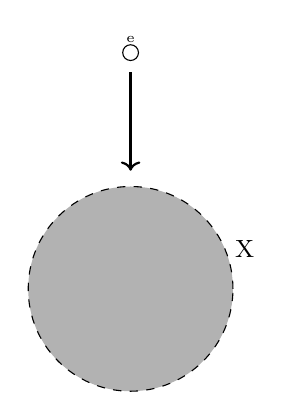
\begin{tikzpicture}
        \draw[dashed,fill=gray!60](0,0) circle(1.3);
        \draw(0,3) circle(0.1) node[above]{\tiny e};
        \draw[thick,->](0,2.75)--(0,1.5);
        \node at (1.45,.5) {\small X};
      \end{tikzpicture}
    \end{center}
    \begin{enumerate}[noitemsep,topsep=0pt,leftmargin=18pt,label=(\Alph*)]
    \item Toward the bottom of the page
    \item Toward the top of the page
    \item Out of the page
    \item Into the page
    \end{enumerate}
  \end{enumerate}

  \columnbreak

  \textbf{Questions 3 and 4}

  \begin{center}
    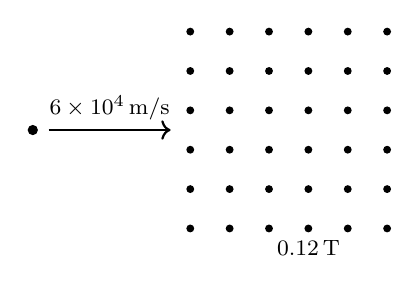
\begin{tikzpicture}[scale=.5]
      \foreach \x in {0,...,5} {
        \foreach \y in {0,...,5} \fill(\x,\y) circle(0.1);
      }
      \node at (3,-.5) {\footnotesize\SI{0.12}{\tesla}};
      \fill[black](-4,2.5) circle(0.13);
      \draw[thick,->](-3.6,2.5)--(-0.5,2.5)
      node[midway,above]{\footnotesize\SI{6e4}{m/s}};
    \end{tikzpicture}
  \end{center}
  A proton is moving at a velocity of \SI{6.0e4}{m/s} to the right, in the
  plane of the page, when it encounters a region of magnetic field with a
  magnitude \SI{0.12}{\tesla} perpendicular to the page, as shown in the
  figure.

  \begin{enumerate}[leftmargin=18pt]
    \setcounter{enumi}{2}
  \item Which of the following is the radius of curvature of the path of the
    proton?
    \begin{enumerate}[noitemsep,topsep=0pt,leftmargin=18pt,label=(\Alph*)]
    \item\SI{5e1}{\metre}
    \item\SI{5e-3}{\metre}
    \item\SI{5e-5}{\metre}
    \item\SI{5e-7}{\metre}
    \end{enumerate}

  \item The proton is replaced with an electron moving in the same direction
    and at the same speed. Which of the following best describes the
    deflection direction and the radius of curvature of the electron in the
    magnetic field?

    \begin{tabular}{lll}
      & \textbf{Deflection direction} & \textbf{Radius of curvature} \\
      \hline
      (A) & Same as proton & Larger than proton's \\
      (B) & Same as proton & Smaller than proton's \\
      (C) & Opposite of proton & Larger than proton's \\
      (D) & Opposite of proton & Smaller than proton's
    \end{tabular}

    \columnbreak

  \item In each of the answer choices below, either a proton or an electron is
    moving toward the top of the page through either an electric or a
    magnetic field. In which case does the charged particle experience a
    force to the right? Select two answers.

    \pic{.45}{screen1.png}

  \item Two long parallel wires carry currents ($I_A$ and $I_B$), as shown in
    the figure. Current $I_A$ in the left wire is twice that of current $I_B$
    in the right wire. The magnetic force on the right wire is $F$. What is the
    magnetic force on the left wire in terms of $F$?
    \begin{center}
      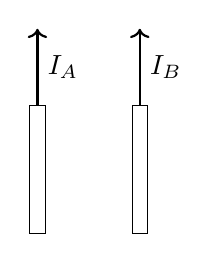
\begin{tikzpicture}[scale=.65]
        \draw(0,.5) rectangle(0.3,3);
        \draw(2,.5) rectangle(2.3,3);
        \draw[thick,->](.15,3)--(.15,4.5) node[midway,right]{$I_A$};;
        \draw[thick,->](2.15,3)--(2.15,4.5) node[midway,right]{$I_B$};;
      \end{tikzpicture}
    \end{center}
    \begin{enumerate}[noitemsep,topsep=0pt,leftmargin=18pt,label=(\Alph*)]
    \item $F$ in the same direction
    \item $F$ in the opposite direction
    \item $F/2$ in the same direction
    \item $F/2$ in the opposite direction
    \end{enumerate}


  \item An iron magnet is broken in half at the midpoint between its north
    and south ends. What is the result?
    \begin{enumerate}[noitemsep,topsep=0pt,leftmargin=18pt,label=(\Alph*)]
    \item A separate north pole and south pole, each with the same magnetic
      strength as the original magnet
    \item A separate north pole and south pole, each with half the magnetic
      strength of the original magnet
    \item Two separate north-south magnets, each with the same magnetic strength
      as the original magnet
    \item Two separate north-south magnets, each with half the magnetic strength
      of the original magnet
    \end{enumerate}

    \columnbreak

  \item The figure shows the microscopic dipoles inside two metal objects.
    Copper is diamagnetic. Iron is ferromagnetic. Which of the following best
    depicts the microscopic internal dipole position when the objects are
    placed in a strong, external magnetic field directed toward the top of the
    page?
    \pic{.45}{screen2.png}
  
  \item Compasses are arranged in a tight circle around a long wire that is
    perpendicular to the plane of the compasses. The wire is represented in
    the figures by a dot. The wire carries a large current directly into the
    page. Which of the following best depicts the orientation of the compass
    needles?
    
    \pic{.45}{screen3.png}
  
    \columnbreak

  \item A magnetic field directed into the page, is placed between two charged
    capacitor plates as shown in the figure. The magnetic and electric fields
    are adjusted so a proton moving at a velocity of $v$ will pass straight
    through the fields. The speed of the proton is doubled to $2v$. Which of
    the following force diagrams most accurately depicts the forces acting on
    the proton when traveling at $2v$?
    \begin{center}
      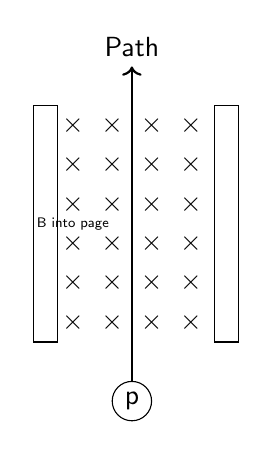
\begin{tikzpicture}
        \draw(0,0) rectangle (.3,3);
        \draw(2.3,0) rectangle (2.6,3);
        \foreach \x in {.5,1,1.5,2}{
          \foreach \y in {0.25,.75,...,2.75} \node at (\x,\y) {$\times$};
        }
        \node at (0.5,1.5){\tiny\textsf{B into page}};
        \draw[thick,->](1.25,-.5)--(1.25,3.5) node[pos=1,above]{\textsf{Path}};
        \draw (1.25,-.75) circle(0.25) node{\textsf{p}};
      \end{tikzpicture}
    \end{center}
    
    \begin{enumerate}[noitemsep,topsep=0pt,leftmargin=18pt,label=(\Alph*)]
    \item\hspace{.4in}\tikz{
      \draw(0,0) circle(.25) node{\textsf{p}};
      \draw[->,thick](.25,0)--(1.25,0);
      \draw[->,thick](-.25,0)--(-1.25,0); }
    \item\hspace{.4in}\tikz{
      \draw(0,0) circle(.25) node{\textsf{p}};
      \draw[->,thick](.25,0)--(2.25,0);
      \draw[->,thick](-.25,0)--(-1.25,0); }
    \item\tikz{
      \draw(0,0) circle(.25) node{\textsf{p}};
      \draw[->,thick](.25,0)--(1.25,0);
      \draw[->,thick](-.25,0)--(-2.25,0); }
    \item\tikz{
      \draw(0,0) circle(.25) node{\textsf{p}};
      \draw[->,thick](.25,0)--(1.25,0);
      \draw[->,thick](-.25,0)--(-2.25,0);
      \draw[->,thick](0,.25)--(0,1.25); }
    \end{enumerate}
  \end{enumerate}

  \columnbreak

  \textbf{Questions 11 and 12}

  An electron is traveling at a constant speed of $v$ parallel to a wire
  carrying a current of $I$, as shown in the figure. The electron is a distance
  of $d$ from the wire.
  \begin{center}
    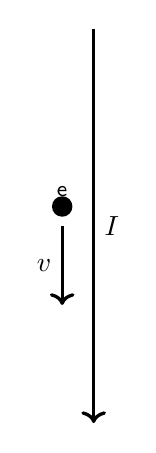
\begin{tikzpicture}
      \draw[very thick,->](0,5)--(0,0) node[midway,right]{$I$};
      \fill[black](-.4,2.75) circle(0.13) node[above]{\footnotesize\textsf{e}};
      \draw[very thick,->](-.4,2.5)--(-.4,1.5) node[midway,left]{$v$};
    \end{tikzpicture}
  \end{center}
  
  \begin{enumerate}[leftmargin=18pt]
    \setcounter{enumi}{10}
  \item Which of the following is true concerning the force on the current-
    carrying wire due to the electron?
    \begin{enumerate}[noitemsep,topsep=0pt,leftmargin=18pt,label=(\Alph*)]
    \item The force is directed toward the right.
    \item The force is directed toward the left.
    \item The force is directed into the page.
    \item There is no force on the current-carrying wire due to the electron.
    \end{enumerate}

  \item The force on the electron from the current is $F$. Which of the
    following will increase the force to $2F$? Select two answers.
    \begin{enumerate}[noitemsep,topsep=0pt,leftmargin=18pt,label=(\Alph*)]
    \item Halve the distance of the electron to the wire.
    \item Halve the velocity of the electron.
    \item Double the current in the wire.
    \item Double the current in the wire and halve the distance of the electron
      to the wire.
    \end{enumerate}
  \end{enumerate}

  \columnbreak

  \textbf{Questions 13 and 14}

  Two wires carry currents $2A$ and $4A$ in the directions shown. Point $P$ is
  a distance $r$ from the wire carrying $2A$, and a distance $2r$ from the wire
  carrying $4A$.
  \begin{center}
    \begin{tikzpicture}[scale=1.2]
      \draw[thick](-.5,0)--(3,0);
      \draw[thick](0,-.5)--(0,3);
      \draw[thick,->](1.5,0)--(2,0) node[pos=1,below]{$4A$};
      \draw[thick,->](0,2)--(0,2.5) node[pos=1,left]{$2A$};
      \draw[dashed](0,2)--(1,2) node[midway,above]{$r$};
      \draw[dashed](1,0)--(1,2) node[midway,right]{$2r$};
      \fill[black](1,2) circle(0.05);
    \end{tikzpicture}
  \end{center}

  \begin{enumerate}[leftmargin=18pt]
    \setcounter{enumi}{12}
  \item Which of the following statements is true?
    \begin{enumerate}[noitemsep,topsep=0pt,leftmargin=18pt,label=(\Alph*)]
    \item The magnetic field produced at point $P$ by the wire carrying $2A$ is
      greater than the magnetic field produced at point $P$ by the wire
      carrying $4A$, but opposite in direction.
    \item The magnetic field produced at point $P$ by the wire carrying $2A$ is
      less than the magnetic field produced at point $P$ by the wire carrying 
      $4A$, and in the same direction.
    \item The magnetic field produced at point $P$ by the wire carrying $2A$ is
      equal to the magnetic field produced at point $P$ by the wire carrying
      $4A$, but opposite in direction.
    \item The magnetic field produced at point $P$ by the wire carrying $2A$ is
      equal to the magnetic field produced at point $P$ by the wire carrying
      $4A$, and in the same direction.
    \item The magnetic field produced at point $P$ by the wire carrying $2A$ is
      greater than the magnetic field produced at point $P$ by the wire
      carrying $4A$, and in the same direction.
    \end{enumerate}

  \item The magnitude of the resultant magnetic field at point $P$ due to the
    current in the two wires is
    \begin{enumerate}[noitemsep,topsep=0pt,leftmargin=18pt,label=(\Alph*)]
    \item zero
    \item $\displaystyle\frac{\mu_0(2A)}{2\pi r}$
    \item $\displaystyle\frac{\mu_0(2A)}{\pi r}$
    \item $\displaystyle\frac{\mu_0(4A)}{2\pi r}$
    \item $\displaystyle\frac{\mu_0(6A)}{4\pi r}$
    \end{enumerate}

    \columnbreak

  \item An electric motor consists of a current-carrying loop of wire mounted
    to an axle and turned at a slight angle in a magnetic field as shown. The
    wire loop will
    
    \pic{.4}{screen5.png}
    \begin{enumerate}[noitemsep,topsep=0pt,leftmargin=18pt,label=(\Alph*)]
    \item experience a torque and turn clockwise
    \item experience a torque and turn counterclockwise
    \item accelerate upward out of the magnetic field
    \item accelerate downward out of the magnetic field
    \item not experience a force or torque
    \end{enumerate}

  \item A current is passed through an analog ammeter and the needle moves
    to indicate the current flowing through the circuit. Which of the
    following best explains how an analog ammeter works?
    \begin{enumerate}[noitemsep,topsep=0pt,leftmargin=18pt,label=(\Alph*)]
    \item Current is passed through the needle placed in a magnetic field, and
      the needle is attracted to the high side of the scale.
    \item The needle is a magnet, and is attracted to a magnet on the high side
      of the scale.
    \item The needle gathers an electrostatic charge from the current, and is
      attracted to an electrostatic charge on the high side of the scale.
    \item Current is passed through a spring coil of wire placed in a magnetic
      field, and the coil rotates, moving the needle proportionally to the
      current in the coil.
    \item Current flows through the needle, making it heavier, and it falls to
      the high side of the scale.
    \end{enumerate}
  \end{enumerate}

  \columnbreak
  
  \textbf{Questions 17 and 18}
  
  A negatively charged particle of mass $m$ and charge $q$ in a uniform
  magnetic field $B$ travels in a circular path of radius $r$.
  \begin{center}
    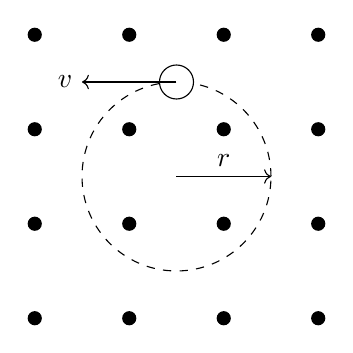
\begin{tikzpicture}[scale=1.2]
      \foreach \x in {0,...,3} {
        \foreach \y in {0,...,3} \fill(\x,\y) circle(0.075);
      }
      \draw[dashed](1.5,1.5) circle(1);
      %\fill(1.5,1.5) circle(0.075);
      \draw[->](1.5,1.5)--(2.5,1.5) node[midway,above]{$r$};
      \draw[fill=white](1.5,2.5) circle(0.18);
      \draw[->](1.5,2.5)--(0.5,2.5) node[pos=1,left]{$v$};
    \end{tikzpicture}
  \end{center}

  \begin{enumerate}[leftmargin=18pt]
    \setcounter{enumi}{16}

  \item In terms of the other given quantities, the charge-to-mass ratio $q/m$
    of the particle is
    \begin{enumerate}[noitemsep,topsep=0pt,leftmargin=18pt,label=(\Alph*)]
    \item $\displaystyle\frac{Bv}{r}$
    \item $\displaystyle\frac{r}{Bv}$
    \item $\displaystyle\frac{rv}{B}$
    \item $rvB$
    \item $\displaystyle\frac{v}{rB}$
    \end{enumerate}
    
  \item The work done by the magnetic field after two full revolutions of the
    charge is
    \begin{enumerate}[noitemsep,topsep=0pt,leftmargin=18pt,label=(\Alph*)]
    \item zero
    \item $-qvB/rm$
    \item $qvm/Br$
    \item $-mBr/qv$
    \item $-mqvBr$
    \end{enumerate}

    \columnbreak
    
%  \item Which of the following graphs best represents the radius $r$ as a
%    functionof magnetic field $B$ for a constant speed?
%    \begin{enumerate}[noitemsep,topsep=0pt,leftmargin=18pt,label=(\Alph*)]
%    \item\tikz{
%      \draw(0,0)--(1,0) node[pos=1,right]{$B$};
%      \draw(0,0)--(0,1) node[pos=1,above]{$r$};
%      \draw(0,0)--(1,0.8);}
%    \item\tikz{
%      \draw(0,0)--(1,0) node[pos=1,right]{$B$};
%      \draw(0,0)--(0,1) node[pos=1,above]{$r$};
%      \addplot {\sqrt{x}};}
%%      \draw[smooth,samples=10,domain=0:1] plot(\sqrt{\x},\x);}
%%    \item\tikz{
%%      \draw(0,0)--(1,0) node[pos=1,right]{$B$};
%%      \draw(0,0)--(0,1) node[pos=1,above]{$r$};
%%      \draw ‎[smooth,samples=10,domain=0:1] plot(\x,‎‎‎‎‎‎‎‎{(\x)...‎‎‎‎‎‎‎‎‎‎‎‎‎‎‎});}
%    \item\tikz{
%      \draw(0,0)--(1,0) node[pos=1,right]{$B$};
%      \draw(0,0)--(0,1) node[pos=1,above]{$r$};
%      \draw(0,.8)--(.8,0);}
%%    \item\tikz{
%%      \draw(0,0)--(1,0) node[pos=1,right]{$B$};
%%      \draw(0,0)--(0,1) node[pos=1,above]{$r$};
%%      \draw ‎[smooth,samples=10,domain=0:1] plot(\x,‎‎‎‎‎‎‎‎{(\x)...‎‎‎‎‎‎‎‎‎‎‎‎‎‎‎});}
%    \end{enumerate}

  \item A stationary compass placed above a charge moving with a speed v
    deflects its needle so that it aligns perpendicular to the velocity of the
    charge. If the compass also moves at the speed v along with the charge,
    the compass will
    \begin{enumerate}[noitemsep,topsep=0pt,leftmargin=18pt,label=(\Alph*)]
    \item deflect \ang{90} relative to the velocity of the charge
    \item deflect \ang{60} relative to the velocity of the charge
    \item deflect \ang{45} relative to the velocity of the charge
    \item deflect \ang{180} relative to the velocity of the charge
    \item not deflect
    \end{enumerate}    
  \end{enumerate}


  \textbf{Questions 20--22}
  
  An electron enters a magnetic field that is directed out of the page as shown.
  The velocity of the electron is to the right.
  \begin{center}
    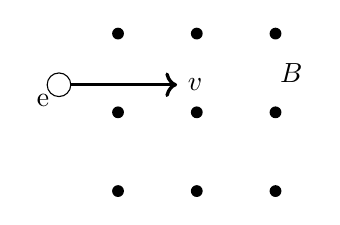
\begin{tikzpicture}
      \foreach \x in {0,...,2} {
        \foreach \y in {0,...,2} \fill(\x,\y) circle(0.075);
      }
      \node at (2.2,1.5) {$B$};
      \draw(-0.75,1.35) circle(0.15) node[below left]{e};
      \draw[very thick,->](-.6,1.35)--(.75,1.35) node[pos=1,right]{$v$};
    \end{tikzpicture}
  \end{center}

  \begin{enumerate}[leftmargin=18pt]
    \setcounter{enumi}{19}
  \item The force the magnetic field exerts on the electron when it enters the
    magnetic field is
    \begin{enumerate}[noitemsep,topsep=0pt,leftmargin=18pt,label=(\Alph*)]
    \item directed into the page
    \item directed out of the page
    \item directed to the top of the page
    \item directed to the bottom of the page
    \item zero
    \end{enumerate}

  \item The resulting path of the electron after entering the magnetic field
    is a
    \begin{enumerate}[noitemsep,topsep=0pt,leftmargin=18pt,label=(\Alph*)]
    \item straight line
    \item circle
    \item spiral
    \item parabola
    \item hyperbola
    \end{enumerate}
    
  \item The work done by the magnetic field on the electron for one complete
    revolution at a radius $r$ is
    \begin{enumerate}[noitemsep,topsep=0pt,leftmargin=18pt,label=(\Alph*)]
    \item $qvBr$
    \item $qvB/r$
    \item $qv/Br$
    \item $Br/qv$
    \item zero
    \end{enumerate}

    \columnbreak

  \item A loop of wire in the plane of the page carries a clockwise current $I$
    and is placed in a magnetic field that is directed into the page as shown.
    Which of the following will happen as a result of the wire loop being in
    the magnetic field?
    \begin{center}
      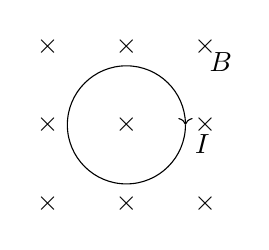
\begin{tikzpicture}
        \foreach \x in {0,...,2} {
          \foreach \y in {0,...,2} \node at (\x,\y) {$\times$};
        }
        \node at (2.2,1.8) {$B$};
        \draw[->](1.75,1) arc(360:0:0.75) node[pos=1,below right]{$I$};
      \end{tikzpicture}
    \end{center}
    \begin{enumerate}[noitemsep,topsep=0pt,leftmargin=18pt,label=(\Alph*)]
    \item The wire loop will rotate clockwise.
    \item The wire loop will rotate counterclockwise.
    \item The wire loop will flip on a horizontal axis through its center.
    \item The wire loop will expand in size.
    \item The wire loop will contract in size.
    \end{enumerate}

    \columnbreak
    
  \item A wire in the plane of the page carries a current directed to the right
    as shown. The wire is placed in a magnetic field that is directed into the
    plane of the page. The force the magnetic field applies to the wire is
    \begin{center}
      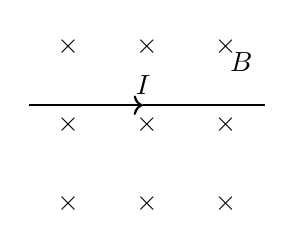
\begin{tikzpicture}
        \foreach \x in {0,...,2} {
          \foreach \y in {0,...,2} \node at (\x,\y) {$\times$};
        }
        \node at (2.2,1.8) {$B$};
        \draw[thick,->](-.5,1.25)--(0.95,1.25) node[pos=1,above]{$I$};
        \draw[thick](0.95,1.25)--(2.5,1.25);
      \end{tikzpicture}
    \end{center}
    \begin{enumerate}[noitemsep,topsep=0pt,leftmargin=18pt,label=(\Alph*)]
    \item directed into the page
    \item directed out of the page
    \item directed to the top of the page
    \item directed to the bottom of the page
    \item zero
    \end{enumerate}
    
  \end{enumerate}
\end{multicols}

\newpage
\begin{center}
  {\Large
    \textbf{AP\textsuperscript{\textregistered} Physics C: Magnetism\\
      Student Answer Sheet for Multiple-Choice Section}
  }
  
  %begin{minipage}{.2\textwidth}
  \vspace{.2in}
  \bgroup
  \begin{tabular}{>{\centering}m{1.3cm} >{\centering}m{1.7cm}}
    No. & Answer
  \end{tabular}\\
  \def\arraystretch{1.5}
  \begin{tabular}{|>{\centering}m{1.3cm}|>{\centering}m{1.7cm}|}
    \hline
    1 & \\ \hline
    2 & \\ \hline
    3 & \\ \hline
    4 & \\ \hline
    5 & \\ \hline
    6 & \\ \hline
    7 & \\ \hline
    8 & \\ \hline
    9 & \\ \hline
    10 & \\ \hline
    11 & \\ \hline
    12 & \\ \hline
    13 & \\ \hline
    14 & \\ \hline
    15 & \\ \hline
    16 & \\ \hline
    17 & \\ \hline
    18 & \\ \hline
    19 & \\ \hline
    20 & \\ \hline
    21 & \\ \hline
    22 & \\ \hline
    23 & \\ \hline
    24 & \\ \hline
  \end{tabular}
  \egroup
  %end{minipage}
\end{center}
\newpage

\genfreetitle{1 \& C}{MAGNETISM}{4}

\genfreedirections{10}

\begin{enumerate}[leftmargin=15pt]

\item A lead box containing radioactive materials that emit both electrons and
  positrons is placed near an apparatus consisting of an evacuated capacitor
  that is filled with a magnetic field, as shown in the figure. Electrons that
  enter along the center line of the capacitor plates travel straight through
  (undeflected) with a velocity of $v=\SI{1.0e7}{m/s}$ and out
  the hole in the center of the apparatus on the right. The capacitor plates
  are separated by a distance of $d=\SI{0.020}{\metre}$; each plate has an area
  of $A=\SI{1.0e-4}{m^2}$ and a potential difference of $\Delta V$. A uniform
  magnetic field of $B=\SI{0.030}{\tesla}$ is directed out of the page between
  the plates, as shown in the figure.

  \vspace{-.2in}
  \begin{center}
    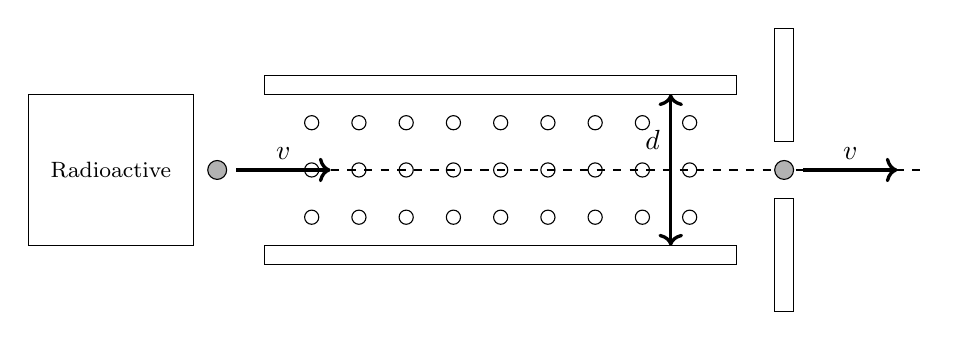
\begin{tikzpicture}[scale=1.2]
      \draw(0,0) rectangle(5,0.2);
      \draw(0,1.8) rectangle(5,2);
      \draw(-.75,0.2) rectangle(-2.5,1.8)
      node[midway]{\footnotesize Radioactive};
      \foreach \x in {.5,1,...,4.5}{
        \foreach \y in {.5,1,1.5} \draw(\x,\y) circle(0.075);
      }
      \draw[dashed](0,1)--(7,1);
      \draw[very thick,<->](4.3,.2)--(4.3,1.8) node[pos=.7,left]{$d$};
      \foreach \xx in {-.5,5.5}{
        \draw[fill=gray!60](\xx,1) circle (0.1);
        \draw[very thick,->](\xx+.2,1)--(\xx+1.2,1) node[midway,above]{$v$};
      }
      \draw(5.4,1.3) rectangle(5.6,2.5);
      \draw(5.4,0.7) rectangle(5.6,-.5);
    \end{tikzpicture}
  \end{center}

  \begin{enumerate}[noitemsep]
  \item\vspace{-.2in} Explain why it is acceptable to neglect the effects of
    gravity on the electrons passing through the apparatus.
  \item
    \begin{enumerate}
    \item Explain why the electrons pass through the capacitor plates
      undeflected. Support your argument with an algebraic equation
      and an appropriately drawn force diagram.

    \item Use your equation to calculate the potential difference ($\Delta V$)
      between the capacitor plates.

    \item Which capacitor plate has the highest potential? Justify your 
      reasoning making reference to the electric field.

    \item Calculate the magnitude of the energy that is stored in the capacitor.
    \end{enumerate}

  \item A positron enters the apparatus along the same path as the
    electrons from part (b).
    \begin{enumerate}
    \item Explain why the positron, traveling at the same speed as the
      electrons, will also travel straight through the device undeflected.
      Support your argument with an equation.
    \item A second positron enters the apparatus at a speed of $2v$. Sketch
      the path of the positron through the capacitor plates on the figure.
    \end{enumerate}

  \item An electron exits the apparatus at a velocity of $v=\SI{1.0e7}{m/s}$
    parallel to a long wire of a circuit, as shown in the figure. The
    distance between the electron and the wire is \SI{1}{mm}.
    \begin{center}
      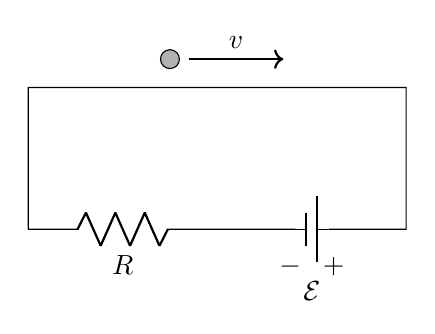
\begin{tikzpicture}[american voltages,scale=1.2]
        \draw(0,-.5)--(0,1)--(4,1)--(4,-.5) to[battery1=$\mathcal{E}$] (2,-.5)
        to[R=$R$] (0,-.5);
        \draw[fill=gray!60](1.5,1.3) circle (0.1);
        \draw[thick,->](1.7,1.3)--(2.7,1.3) node[midway,above]{$v$};
      \end{tikzpicture}
    \end{center}
    \begin{enumerate}
    \item Calculate the potential difference-to-resistance ratio of the circuit
      such that the electron will experience a force $F$ of \SI{1.3e-16}{N}.
    \item Draw a force vector on the figure to show the direction of the force
      on the electron.
    \end{enumerate}
  \end{enumerate}
\end{enumerate}
\newpage
Perform calculations for Question 1 here.
\newpage

\begin{center}
  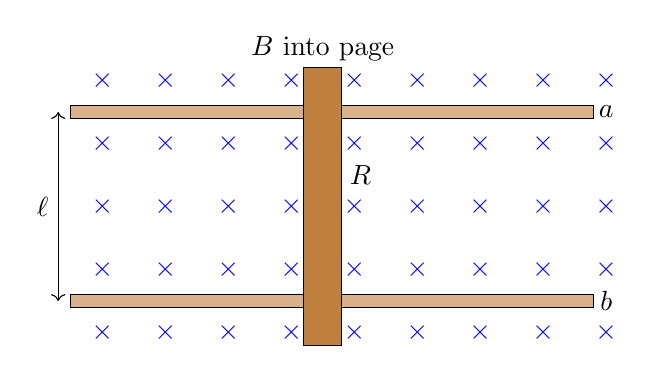
\begin{tikzpicture}[scale=.8]
    \foreach \x in {0,...,8} {
      \foreach \y in {0,...,4} \node at (\x,\y) {\textcolor{blue}{$\times$}};
    }
    \draw[fill=brown!60](-.5,3.4) rectangle(7.8,3.6);
    \draw[fill=brown!60](-.5,0.4) rectangle(7.8,0.6);
    \draw[fill=brown](3.2,-.2) rectangle(3.8,4.2);
    \draw[<->](-0.7,0.5)--(-0.7,3.5) node[midway,left]{$\ell$};
    \node at (3.5,4.5) {$\mb{B}$ into page};
    \node at (8,0.5) {$b$};
    \node at (8,3.5) {$a$};
    \node at (4.1,2.5) {$R$};
  \end{tikzpicture}
\end{center}

\begin{enumerate}[leftmargin=18pt]
  \setcounter{enumi}{1}
\item In the above figure, a rod has a resistance and the rails have negligible
  resistance. A battery of emf $\mathcal{E}$ and negligible internal resistance
  is connected between points $a$ and $b$ such that the current in the rod is
  downward. The rod is placed at rest aqt $t=0$.
  \begin{enumerate}[noitemsep]
  \item Find the force on the rod as a function of speed $v$.
  \item Show that the rod reaches terminal velocity, and find the expression for
    it.
  \item What is the current when the rod reaches its terminal velocity?
  \end{enumerate}
  \vspace{2in}
  
\item In the above figure, the rod has a resistance of $R$ and the rails have
  negligible resistance. A capacitor with charge $Q_0$ and capacitance $C$ is
  connected between points $a$ and $b$ such that the current in the road is
  downward. The rod is places at rest at $t=0$.
  \begin{enumerate}[noitemsep]
  \item Write the equation of motion for the rod on the rails.
  \item Show that the terminal speed of the rod down the rail is related to the
    final charge on the capacitor.
  \end{enumerate}
\end{enumerate}
\newpage
\begin{center}
  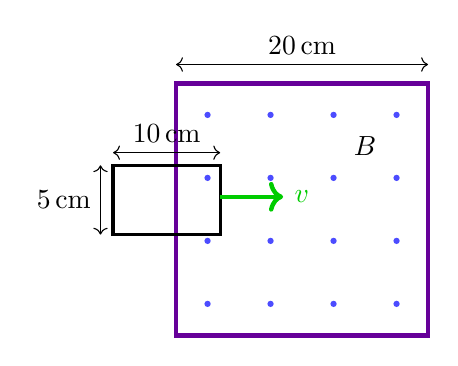
\begin{tikzpicture}[scale=.8]
    \draw[blue!60!red,ultra thick](0,0) rectangle(4,4);
    \draw[<->](0,4.3)--(4,4.3) node[midway,above]{\SI{20}{cm}};
    \foreach \x in {0.5,1.5,...,3.5} {
      \foreach \y in {0.5,1.5,...,3.5} \fill[blue!70](\x,\y) circle(0.05);
    }
    \node at (3,3) {$\mb{B}$};
    \draw[very thick](-1,1.6) rectangle(0.7,2.7);
    \draw[<->](-1.2,1.6)--(-1.2,2.7) node[midway,left]{\SI{5}{cm}};
    \draw[<->](-1,2.9)--(.7,2.9) node[midway,above]{\SI{10}{cm}};
    \draw[green!80!black,ultra thick,->](.7,2.2)--(1.7,2.2)
    node[pos=1,right]{$v$};
  \end{tikzpicture} 
\end{center}

\begin{enumerate}[leftmargin=18pt]

  \setcounter{enumi}{3}
\item A \SI{10}{cm} by \SI{5}{cm} rectangular loop with resistance
  \SI{2.5}{\ohm} is pulled through a region of uniform magnetic field
  $B=\SI{1.7}{\tesla}$ with constant speed $v=\SI{2.4}{cm/s}$. The front of the
  loop enters the region of the magnetic field at time $t=0$.
  \begin{enumerate}[noitemsep,leftmargin=18pt]
  \item Find and graph the flux through the loop as a function of time.
  \item Find and graph the included emf and the current in the loop as a
    function of time. Neglect any self inductance of the loop and extend your
    graph from $t=0$ to $t=\SI{16}{\second}$.
  \end{enumerate}
\end{enumerate}
\end{document}
